\documentclass[1p]{elsarticle_modified}
%\bibliographystyle{elsarticle-num}

%\usepackage[colorlinks]{hyperref}
%\usepackage{abbrmath_seonhwa} %\Abb, \Ascr, \Acal ,\Abf, \Afrak
\usepackage{amsfonts}
\usepackage{amssymb}
\usepackage{amsmath}
\usepackage{amsthm}
\usepackage{scalefnt}
\usepackage{amsbsy}
\usepackage{kotex}
\usepackage{caption}
\usepackage{subfig}
\usepackage{color}
\usepackage{graphicx}
\usepackage{xcolor} %% white, black, red, green, blue, cyan, magenta, yellow
\usepackage{float}
\usepackage{setspace}
\usepackage{hyperref}

\usepackage{tikz}
\usetikzlibrary{arrows}

\usepackage{multirow}
\usepackage{array} % fixed length table
\usepackage{hhline}

%%%%%%%%%%%%%%%%%%%%%
\makeatletter
\renewcommand*\env@matrix[1][\arraystretch]{%
	\edef\arraystretch{#1}%
	\hskip -\arraycolsep
	\let\@ifnextchar\new@ifnextchar
	\array{*\c@MaxMatrixCols c}}
\makeatother %https://tex.stackexchange.com/questions/14071/how-can-i-increase-the-line-spacing-in-a-matrix
%%%%%%%%%%%%%%%

\usepackage[normalem]{ulem}

\newcommand{\msout}[1]{\ifmmode\text{\sout{\ensuremath{#1}}}\else\sout{#1}\fi}
%SOURCE: \msout is \stkout macro in https://tex.stackexchange.com/questions/20609/strikeout-in-math-mode

\newcommand{\cancel}[1]{
	\ifmmode
	{\color{red}\msout{#1}}
	\else
	{\color{red}\sout{#1}}
	\fi
}

\newcommand{\add}[1]{
	{\color{blue}\uwave{#1}}
}

\newcommand{\replace}[2]{
	\ifmmode
	{\color{red}\msout{#1}}{\color{blue}\uwave{#2}}
	\else
	{\color{red}\sout{#1}}{\color{blue}\uwave{#2}}
	\fi
}

\newcommand{\Sol}{\mathcal{S}} %segment
\newcommand{\D}{D} %diagram
\newcommand{\A}{\mathcal{A}} %arc


%%%%%%%%%%%%%%%%%%%%%%%%%%%%%5 test

\def\sl{\operatorname{\textup{SL}}(2,\Cbb)}
\def\psl{\operatorname{\textup{PSL}}(2,\Cbb)}
\def\quan{\mkern 1mu \triangleright \mkern 1mu}

\theoremstyle{definition}
\newtheorem{thm}{Theorem}[section]
\newtheorem{prop}[thm]{Proposition}
\newtheorem{lem}[thm]{Lemma}
\newtheorem{ques}[thm]{Question}
\newtheorem{cor}[thm]{Corollary}
\newtheorem{defn}[thm]{Definition}
\newtheorem{exam}[thm]{Example}
\newtheorem{rmk}[thm]{Remark}
\newtheorem{alg}[thm]{Algorithm}

\newcommand{\I}{\sqrt{-1}}
\begin{document}

%\begin{frontmatter}
%
%\title{Boundary parabolic representations of knots up to 8 crossings}
%
%%% Group authors per affiliation:
%\author{Yunhi Cho} 
%\address{Department of Mathematics, University of Seoul, Seoul, Korea}
%\ead{yhcho@uos.ac.kr}
%
%
%\author{Seonhwa Kim} %\fnref{s_kim}}
%\address{Center for Geometry and Physics, Institute for Basic Science, Pohang, 37673, Korea}
%\ead{ryeona17@ibs.re.kr}
%
%\author{Hyuk Kim}
%\address{Department of Mathematical Sciences, Seoul National University, Seoul 08826, Korea}
%\ead{hyukkim@snu.ac.kr}
%
%\author{Seokbeom Yoon}
%\address{Department of Mathematical Sciences, Seoul National University, Seoul, 08826,  Korea}
%\ead{sbyoon15@snu.ac.kr}
%
%\begin{abstract}
%We find all boundary parabolic representation of knots up to 8 crossings.
%
%\end{abstract}
%\begin{keyword}
%    \MSC[2010] 57M25 
%\end{keyword}
%
%\end{frontmatter}

%\linenumbers
%\tableofcontents
%
\newcommand\colored[1]{\textcolor{white}{\rule[-0.35ex]{0.8em}{1.4ex}}\kern-0.8em\color{red} #1}%
%\newcommand\colored[1]{\textcolor{white}{ #1}\kern-2.17ex	\textcolor{white}{ #1}\kern-1.81ex	\textcolor{white}{ #1}\kern-2.15ex\color{red}#1	}

{\Large $\underline{11a_{288}~(K11a_{288})}$}

\setlength{\tabcolsep}{10pt}
\renewcommand{\arraystretch}{1.6}
\vspace{1cm}\begin{tabular}{m{100pt}>{\centering\arraybackslash}m{274pt}}
\multirow{5}{120pt}{
	\centering
	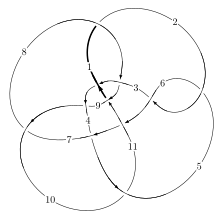
\includegraphics[width=112pt]{../../../GIT/diagram.site/Diagrams/png/537_11a_288.png}\\
\ \ \ A knot diagram\footnotemark}&
\allowdisplaybreaks
\textbf{Linearized knot diagam} \\
\cline{2-2}
 &
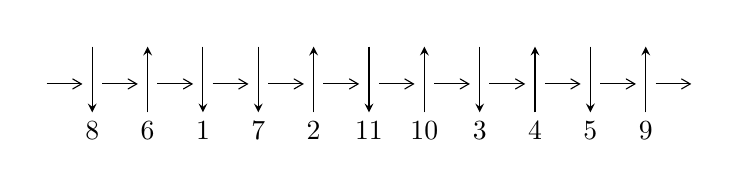
\begin{tikzpicture}[x=20pt, y=17pt]
	% nodes
	\node (C0) at (0, 0) {};
	\node (C1) at (1, 0) {};
	\node (C1U) at (1, +1) {};
	\node (C1D) at (1, -1) {8};

	\node (C2) at (2, 0) {};
	\node (C2U) at (2, +1) {};
	\node (C2D) at (2, -1) {6};

	\node (C3) at (3, 0) {};
	\node (C3U) at (3, +1) {};
	\node (C3D) at (3, -1) {1};

	\node (C4) at (4, 0) {};
	\node (C4U) at (4, +1) {};
	\node (C4D) at (4, -1) {7};

	\node (C5) at (5, 0) {};
	\node (C5U) at (5, +1) {};
	\node (C5D) at (5, -1) {2};

	\node (C6) at (6, 0) {};
	\node (C6U) at (6, +1) {};
	\node (C6D) at (6, -1) {11};

	\node (C7) at (7, 0) {};
	\node (C7U) at (7, +1) {};
	\node (C7D) at (7, -1) {10};

	\node (C8) at (8, 0) {};
	\node (C8U) at (8, +1) {};
	\node (C8D) at (8, -1) {3};

	\node (C9) at (9, 0) {};
	\node (C9U) at (9, +1) {};
	\node (C9D) at (9, -1) {4};

	\node (C10) at (10, 0) {};
	\node (C10U) at (10, +1) {};
	\node (C10D) at (10, -1) {5};

	\node (C11) at (11, 0) {};
	\node (C11U) at (11, +1) {};
	\node (C11D) at (11, -1) {9};
	\node (C12) at (12, 0) {};

	% arrows
	\draw[->,>={angle 60}]
	(C0) edge (C1) (C1) edge (C2) (C2) edge (C3) (C3) edge (C4) (C4) edge (C5) (C5) edge (C6) (C6) edge (C7) (C7) edge (C8) (C8) edge (C9) (C9) edge (C10) (C10) edge (C11) (C11) edge (C12) ;	\draw[->,>=stealth]
	(C1U) edge (C1D) (C2D) edge (C2U) (C3U) edge (C3D) (C4U) edge (C4D) (C5D) edge (C5U) (C6U) edge (C6D) (C7D) edge (C7U) (C8U) edge (C8D) (C9D) edge (C9U) (C10U) edge (C10D) (C11D) edge (C11U) ;
	\end{tikzpicture} \\
\hhline{~~} \\& 
\textbf{Solving Sequence} \\ \cline{2-2} 
 &
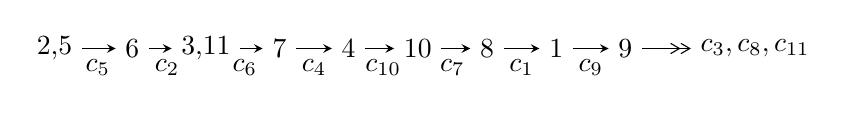
\begin{tikzpicture}[x=25pt, y=7pt]
	% node
	\node (A0) at (-1/8, 0) {2,5};
	\node (A1) at (1, 0) {6};
	\node (A2) at (33/16, 0) {3,11};
	\node (A3) at (25/8, 0) {7};
	\node (A4) at (33/8, 0) {4};
	\node (A5) at (41/8, 0) {10};
	\node (A6) at (49/8, 0) {8};
	\node (A7) at (57/8, 0) {1};
	\node (A8) at (65/8, 0) {9};
	\node (C1) at (1/2, -1) {$c_{5}$};
	\node (C2) at (3/2, -1) {$c_{2}$};
	\node (C3) at (21/8, -1) {$c_{6}$};
	\node (C4) at (29/8, -1) {$c_{4}$};
	\node (C5) at (37/8, -1) {$c_{10}$};
	\node (C6) at (45/8, -1) {$c_{7}$};
	\node (C7) at (53/8, -1) {$c_{1}$};
	\node (C8) at (61/8, -1) {$c_{9}$};
	\node (A9) at (10, 0) {$c_{3},c_{8},c_{11}$};

	% edge
	\draw[->,>=stealth]	
	(A0) edge (A1) (A1) edge (A2) (A2) edge (A3) (A3) edge (A4) (A4) edge (A5) (A5) edge (A6) (A6) edge (A7) (A7) edge (A8) ;
	\draw[->>,>={angle 60}]	
	(A8) edge (A9);
\end{tikzpicture} \\ 

\end{tabular} \\

\footnotetext{
The image of knot diagram is generated by the software ``\textbf{Draw programme}" developed by Andrew Bartholomew(\url{http://www.layer8.co.uk/maths/draw/index.htm\#Running-draw}), where we modified some parts for our purpose(\url{https://github.com/CATsTAILs/LinksPainter}).
}\phantom \\ \newline 
\centering \textbf{Ideals for irreducible components\footnotemark of $X_{\text{par}}$} 
 
\begin{align*}
I^u_{1}&=\langle 
8.06723\times10^{36} u^{30}-2.15815\times10^{37} u^{29}+\cdots+3.48049\times10^{38} b+2.48334\times10^{38},\\
\phantom{I^u_{1}}&\phantom{= \langle  }2.80307\times10^{38} u^{30}-9.56905\times10^{38} u^{29}+\cdots+4.87269\times10^{39} a+9.46071\times10^{39},\;u^{31}-4 u^{30}+\cdots+50 u-28\rangle \\
I^u_{2}&=\langle 
-2.07446\times10^{51} a u^{49}-3.96254\times10^{51} u^{49}+\cdots+1.37652\times10^{52} a+2.97634\times10^{52},\\
\phantom{I^u_{2}}&\phantom{= \langle  }1.89907\times10^{50} a u^{49}+3.15834\times10^{50} u^{49}+\cdots-1.33112\times10^{51} a-2.21453\times10^{51},\;u^{50}+u^{49}+\cdots+53 u^2-5\rangle \\
I^u_{3}&=\langle 
-120 u^{11} a-53 u^{11}+\cdots+159 a-21,\;2244 u^{11} a-88 u^{11}+\cdots-4869 a+704,\\
\phantom{I^u_{3}}&\phantom{= \langle  }u^{12}-2 u^{10}- u^8+8 u^6-2 u^5-10 u^4+5 u^3+6 u^2- u-1\rangle \\
I^u_{4}&=\langle 
- u^3+u^2+b-1,\;-2 u^4+2 u^3+u^2+a-2 u-2,\;u^5- u^4- u^3+2 u^2+u-1\rangle \\
\\
\end{align*}
\raggedright * 4 irreducible components of $\dim_{\mathbb{C}}=0$, with total 160 representations.\\
\footnotetext{All coefficients of polynomials are rational numbers. But the coefficients are sometimes approximated in decimal forms when there is not enough margin.}
\newpage
\renewcommand{\arraystretch}{1}
\centering \section*{I. $I^u_{1}= \langle 8.07\times10^{36} u^{30}-2.16\times10^{37} u^{29}+\cdots+3.48\times10^{38} b+2.48\times10^{38},\;2.80\times10^{38} u^{30}-9.57\times10^{38} u^{29}+\cdots+4.87\times10^{39} a+9.46\times10^{39},\;u^{31}-4 u^{30}+\cdots+50 u-28 \rangle$}
\flushleft \textbf{(i) Arc colorings}\\
\begin{tabular}{m{7pt} m{180pt} m{7pt} m{180pt} }
\flushright $a_{2}=$&$\begin{pmatrix}0\\u\end{pmatrix}$ \\
\flushright $a_{5}=$&$\begin{pmatrix}1\\0\end{pmatrix}$ \\
\flushright $a_{6}=$&$\begin{pmatrix}1\\- u^2\end{pmatrix}$ \\
\flushright $a_{3}=$&$\begin{pmatrix}u\\- u^3+u\end{pmatrix}$ \\
\flushright $a_{11}=$&$\begin{pmatrix}-0.0575261 u^{30}+0.196381 u^{29}+\cdots-0.668017 u-1.94158\\-0.0231784 u^{30}+0.0620070 u^{29}+\cdots-1.21996 u-0.713504\end{pmatrix}$ \\
\flushright $a_{7}=$&$\begin{pmatrix}0.176167 u^{30}-0.581968 u^{29}+\cdots-3.39968 u+7.23962\\0.0343023 u^{30}-0.100932 u^{29}+\cdots+0.798398 u+0.793988\end{pmatrix}$ \\
\flushright $a_{4}=$&$\begin{pmatrix}-0.208417 u^{30}+0.691487 u^{29}+\cdots+2.50241 u-7.53909\\-0.0519901 u^{30}+0.176388 u^{29}+\cdots+1.60836 u-1.85459\end{pmatrix}$ \\
\flushright $a_{10}=$&$\begin{pmatrix}-0.0807046 u^{30}+0.258388 u^{29}+\cdots-1.88798 u-2.65508\\-0.0231784 u^{30}+0.0620070 u^{29}+\cdots-1.21996 u-0.713504\end{pmatrix}$ \\
\flushright $a_{8}=$&$\begin{pmatrix}0.0592055 u^{30}-0.204794 u^{29}+\cdots-3.84139 u+4.10481\\0.00850606 u^{30}-0.0427335 u^{29}+\cdots-0.991100 u+0.713957\end{pmatrix}$ \\
\flushright $a_{1}=$&$\begin{pmatrix}0.151056 u^{30}-0.489997 u^{29}+\cdots-0.795159 u+7.14890\\0.0373762 u^{30}-0.128110 u^{29}+\cdots-0.0869666 u+1.73434\end{pmatrix}$ \\
\flushright $a_{9}=$&$\begin{pmatrix}0.0899122 u^{30}-0.296684 u^{29}+\cdots-4.28680 u+4.75380\\0.0118652 u^{30}-0.0465465 u^{29}+\cdots-0.749425 u+0.496701\end{pmatrix}$\\ \flushright $a_{9}=$&$\begin{pmatrix}0.0899122 u^{30}-0.296684 u^{29}+\cdots-4.28680 u+4.75380\\0.0118652 u^{30}-0.0465465 u^{29}+\cdots-0.749425 u+0.496701\end{pmatrix}$\\&\end{tabular}
\flushleft \textbf{(ii) Obstruction class $= -1$}\\~\\
\flushleft \textbf{(iii) Cusp Shapes $= -0.171373 u^{30}+0.572368 u^{29}+\cdots-0.551385 u-4.18306$}\\~\\
\newpage\renewcommand{\arraystretch}{1}
\flushleft \textbf{(iv) u-Polynomials at the component}\newline \\
\begin{tabular}{m{50pt}|m{274pt}}
Crossings & \hspace{64pt}u-Polynomials at each crossing \\
\hline $$\begin{aligned}c_{1},c_{6}\end{aligned}$$&$\begin{aligned}
&u^{31}-7 u^{30}+\cdots+96 u-12
\end{aligned}$\\
\hline $$\begin{aligned}c_{2},c_{5}\end{aligned}$$&$\begin{aligned}
&u^{31}-4 u^{30}+\cdots+50 u-28
\end{aligned}$\\
\hline $$\begin{aligned}c_{3},c_{4}\end{aligned}$$&$\begin{aligned}
&u^{31}-2 u^{30}+\cdots-9 u+3
\end{aligned}$\\
\hline $$\begin{aligned}c_{7},c_{11}\end{aligned}$$&$\begin{aligned}
&u^{31}-4 u^{30}+\cdots-3 u-1
\end{aligned}$\\
\hline $$\begin{aligned}c_{8},c_{10}\end{aligned}$$&$\begin{aligned}
&3(3 u^{31}-6 u^{30}+\cdots+5 u-1)
\end{aligned}$\\
\hline $$\begin{aligned}c_{9}\end{aligned}$$&$\begin{aligned}
&3(3 u^{31}+9 u^{30}+\cdots+832 u+128)
\end{aligned}$\\
\hline
\end{tabular}\\~\\
\newpage\renewcommand{\arraystretch}{1}
\flushleft \textbf{(v) Riley Polynomials at the component}\newline \\
\begin{tabular}{m{50pt}|m{274pt}}
Crossings & \hspace{64pt}Riley Polynomials at each crossing \\
\hline $$\begin{aligned}c_{1},c_{6}\end{aligned}$$&$\begin{aligned}
&y^{31}+5 y^{30}+\cdots-1776 y-144
\end{aligned}$\\
\hline $$\begin{aligned}c_{2},c_{5}\end{aligned}$$&$\begin{aligned}
&y^{31}-12 y^{30}+\cdots-7860 y-784
\end{aligned}$\\
\hline $$\begin{aligned}c_{3},c_{4}\end{aligned}$$&$\begin{aligned}
&y^{31}-6 y^{30}+\cdots+51 y-9
\end{aligned}$\\
\hline $$\begin{aligned}c_{7},c_{11}\end{aligned}$$&$\begin{aligned}
&y^{31}+2 y^{30}+\cdots+3 y-1
\end{aligned}$\\
\hline $$\begin{aligned}c_{8},c_{10}\end{aligned}$$&$\begin{aligned}
&9(9 y^{31}+120 y^{30}+\cdots+9 y-1)
\end{aligned}$\\
\hline $$\begin{aligned}c_{9}\end{aligned}$$&$\begin{aligned}
&9(9 y^{31}+57 y^{30}+\cdots+331776 y-16384)
\end{aligned}$\\
\hline
\end{tabular}\\~\\
\newpage\flushleft \textbf{(vi) Complex Volumes and Cusp Shapes}
$$\begin{array}{c|c|c}  
\text{Solutions to }I^u_{1}& \I (\text{vol} + \sqrt{-1}CS) & \text{Cusp shape}\\
 \hline 
\begin{aligned}
u &= -0.902043 + 0.474320 I \\
a &= -1.36116 + 0.92502 I \\
b &= -0.249318 - 0.764075 I\end{aligned}
 & \phantom{-}3.74146 - 4.83276 I & \phantom{-}8.35445 + 8.23935 I \\ \hline\begin{aligned}
u &= -0.902043 - 0.474320 I \\
a &= -1.36116 - 0.92502 I \\
b &= -0.249318 + 0.764075 I\end{aligned}
 & \phantom{-}3.74146 + 4.83276 I & \phantom{-}8.35445 - 8.23935 I \\ \hline\begin{aligned}
u &= \phantom{-}1.005070 + 0.357655 I \\
a &= \phantom{-}0.56639 + 1.94456 I \\
b &= \phantom{-}0.045950 - 1.405710 I\end{aligned}
 & \phantom{-}4.44624 + 0.88533 I & \phantom{-}2.97033 - 0.43256 I \\ \hline\begin{aligned}
u &= \phantom{-}1.005070 - 0.357655 I \\
a &= \phantom{-}0.56639 - 1.94456 I \\
b &= \phantom{-}0.045950 + 1.405710 I\end{aligned}
 & \phantom{-}4.44624 - 0.88533 I & \phantom{-}2.97033 + 0.43256 I \\ \hline\begin{aligned}
u &= \phantom{-}0.396207 + 1.023040 I \\
a &= -0.134995 + 0.574699 I \\
b &= -0.276299 + 0.112521 I\end{aligned}
 & -2.52139 + 3.24553 I & -8.21889 - 3.28316 I \\ \hline\begin{aligned}
u &= \phantom{-}0.396207 - 1.023040 I \\
a &= -0.134995 - 0.574699 I \\
b &= -0.276299 - 0.112521 I\end{aligned}
 & -2.52139 - 3.24553 I & -8.21889 + 3.28316 I \\ \hline\begin{aligned}
u &= -0.304429 + 1.124820 I \\
a &= \phantom{-}0.038514 + 0.323938 I \\
b &= -0.820173 + 1.047500 I\end{aligned}
 & -3.41746 + 4.90251 I & -7.14123 - 8.81153 I \\ \hline\begin{aligned}
u &= -0.304429 - 1.124820 I \\
a &= \phantom{-}0.038514 - 0.323938 I \\
b &= -0.820173 - 1.047500 I\end{aligned}
 & -3.41746 - 4.90251 I & -7.14123 + 8.81153 I \\ \hline\begin{aligned}
u &= -1.073900 + 0.514023 I \\
a &= -0.42433 + 1.48714 I \\
b &= -0.668135 - 0.446989 I\end{aligned}
 & \phantom{-}0.39997 - 5.14043 I & -3.97875 + 8.74276 I \\ \hline\begin{aligned}
u &= -1.073900 - 0.514023 I \\
a &= -0.42433 - 1.48714 I \\
b &= -0.668135 + 0.446989 I\end{aligned}
 & \phantom{-}0.39997 + 5.14043 I & -3.97875 - 8.74276 I\\
 \hline 
 \end{array}$$\newpage$$\begin{array}{c|c|c}  
\text{Solutions to }I^u_{1}& \I (\text{vol} + \sqrt{-1}CS) & \text{Cusp shape}\\
 \hline 
\begin{aligned}
u &= \phantom{-}0.360300 + 1.182790 I \\
a &= \phantom{-}0.1307640 - 0.0393439 I \\
b &= \phantom{-}1.02402 + 0.99307 I\end{aligned}
 & \phantom{-}0.34389 - 13.57870 I & -0.70654 + 8.53646 I \\ \hline\begin{aligned}
u &= \phantom{-}0.360300 - 1.182790 I \\
a &= \phantom{-}0.1307640 + 0.0393439 I \\
b &= \phantom{-}1.02402 - 0.99307 I\end{aligned}
 & \phantom{-}0.34389 + 13.57870 I & -0.70654 - 8.53646 I \\ \hline\begin{aligned}
u &= \phantom{-}1.161460 + 0.451121 I \\
a &= -0.090591 + 1.372090 I \\
b &= \phantom{-}0.330471 - 0.343611 I\end{aligned}
 & \phantom{-}0.48261 + 1.92668 I & -1.89690 + 0.93654 I \\ \hline\begin{aligned}
u &= \phantom{-}1.161460 - 0.451121 I \\
a &= -0.090591 - 1.372090 I \\
b &= \phantom{-}0.330471 + 0.343611 I\end{aligned}
 & \phantom{-}0.48261 - 1.92668 I & -1.89690 - 0.93654 I \\ \hline\begin{aligned}
u &= -0.417016 + 0.598371 I \\
a &= \phantom{-}0.699354 + 0.161448 I \\
b &= \phantom{-}0.733122 - 0.200454 I\end{aligned}
 & -1.51628 + 0.70429 I & -5.99175 - 2.53077 I \\ \hline\begin{aligned}
u &= -0.417016 - 0.598371 I \\
a &= \phantom{-}0.699354 - 0.161448 I \\
b &= \phantom{-}0.733122 + 0.200454 I\end{aligned}
 & -1.51628 - 0.70429 I & -5.99175 + 2.53077 I \\ \hline\begin{aligned}
u &= \phantom{-}0.723629\phantom{ +0.000000I} \\
a &= -2.83794\phantom{ +0.000000I} \\
b &= -0.817850\phantom{ +0.000000I}\end{aligned}
 & -2.61872\phantom{ +0.000000I} & -6.04380\phantom{ +0.000000I} \\ \hline\begin{aligned}
u &= \phantom{-}1.294070 + 0.080005 I \\
a &= \phantom{-}0.001044 - 1.343360 I \\
b &= -0.37710 + 1.64204 I\end{aligned}
 & \phantom{-}3.31474 - 0.89260 I & -5.46909 + 7.98486 I \\ \hline\begin{aligned}
u &= \phantom{-}1.294070 - 0.080005 I \\
a &= \phantom{-}0.001044 + 1.343360 I \\
b &= -0.37710 - 1.64204 I\end{aligned}
 & \phantom{-}3.31474 + 0.89260 I & -5.46909 - 7.98486 I \\ \hline\begin{aligned}
u &= \phantom{-}0.378286 + 1.348700 I \\
a &= \phantom{-}0.203259 + 0.019001 I \\
b &= \phantom{-}0.178022 - 0.791454 I\end{aligned}
 & -0.69495 + 3.65306 I & \phantom{-}9.41146 - 5.59206 I\\
 \hline 
 \end{array}$$\newpage$$\begin{array}{c|c|c}  
\text{Solutions to }I^u_{1}& \I (\text{vol} + \sqrt{-1}CS) & \text{Cusp shape}\\
 \hline 
\begin{aligned}
u &= \phantom{-}0.378286 - 1.348700 I \\
a &= \phantom{-}0.203259 - 0.019001 I \\
b &= \phantom{-}0.178022 + 0.791454 I\end{aligned}
 & -0.69495 - 3.65306 I & \phantom{-}9.41146 + 5.59206 I \\ \hline\begin{aligned}
u &= -1.261620 + 0.633674 I \\
a &= \phantom{-}0.30551 - 1.50157 I \\
b &= \phantom{-}1.27831 + 1.31389 I\end{aligned}
 & -0.34268 - 11.10620 I & -2.89392 + 11.18360 I \\ \hline\begin{aligned}
u &= -1.261620 - 0.633674 I \\
a &= \phantom{-}0.30551 + 1.50157 I \\
b &= \phantom{-}1.27831 - 1.31389 I\end{aligned}
 & -0.34268 + 11.10620 I & -2.89392 - 11.18360 I \\ \hline\begin{aligned}
u &= \phantom{-}1.27757 + 0.69297 I \\
a &= -0.37637 - 1.58211 I \\
b &= -1.22288 + 1.11044 I\end{aligned}
 & \phantom{-}3.2833 + 20.2067 I & \phantom{-}1.01289 - 10.64976 I \\ \hline\begin{aligned}
u &= \phantom{-}1.27757 - 0.69297 I \\
a &= -0.37637 + 1.58211 I \\
b &= -1.22288 - 1.11044 I\end{aligned}
 & \phantom{-}3.2833 - 20.2067 I & \phantom{-}1.01289 + 10.64976 I \\ \hline\begin{aligned}
u &= \phantom{-}1.31560 + 0.78153 I \\
a &= \phantom{-}0.197901 + 0.676665 I \\
b &= \phantom{-}0.297387 - 0.693752 I\end{aligned}
 & \phantom{-}2.20531 + 3.28606 I & \phantom{-}18.4949 - 4.2675 I \\ \hline\begin{aligned}
u &= \phantom{-}1.31560 - 0.78153 I \\
a &= \phantom{-}0.197901 - 0.676665 I \\
b &= \phantom{-}0.297387 + 0.693752 I\end{aligned}
 & \phantom{-}2.20531 - 3.28606 I & \phantom{-}18.4949 + 4.2675 I \\ \hline\begin{aligned}
u &= -1.56081 + 0.05643 I \\
a &= \phantom{-}0.404127 - 0.969867 I \\
b &= -0.581198 + 1.166820 I\end{aligned}
 & \phantom{-}7.70413 + 8.70305 I & \phantom{-}5.79340 - 7.62622 I \\ \hline\begin{aligned}
u &= -1.56081 - 0.05643 I \\
a &= \phantom{-}0.404127 + 0.969867 I \\
b &= -0.581198 - 1.166820 I\end{aligned}
 & \phantom{-}7.70413 - 8.70305 I & \phantom{-}5.79340 + 7.62622 I \\ \hline\begin{aligned}
u &= -0.030538 + 0.374368 I \\
a &= \phantom{-}0.723845 - 0.624919 I \\
b &= -0.283244 - 0.791915 I\end{aligned}
 & \phantom{-}1.97471 + 1.86806 I & \phantom{-}2.78153 - 1.05232 I\\
 \hline 
 \end{array}$$\newpage$$\begin{array}{c|c|c}  
\text{Solutions to }I^u_{1}& \I (\text{vol} + \sqrt{-1}CS) & \text{Cusp shape}\\
 \hline 
\begin{aligned}
u &= -0.030538 - 0.374368 I \\
a &= \phantom{-}0.723845 + 0.624919 I \\
b &= -0.283244 + 0.791915 I\end{aligned}
 & \phantom{-}1.97471 - 1.86806 I & \phantom{-}2.78153 + 1.05232 I\\
 \hline 
 \end{array}$$\newpage\newpage\renewcommand{\arraystretch}{1}
\centering \section*{II. $I^u_{2}= \langle -2.07\times10^{51} a u^{49}-3.96\times10^{51} u^{49}+\cdots+1.38\times10^{52} a+2.98\times10^{52},\;1.90\times10^{50} a u^{49}+3.16\times10^{50} u^{49}+\cdots-1.33\times10^{51} a-2.21\times10^{51},\;u^{50}+u^{49}+\cdots+53 u^2-5 \rangle$}
\flushleft \textbf{(i) Arc colorings}\\
\begin{tabular}{m{7pt} m{180pt} m{7pt} m{180pt} }
\flushright $a_{2}=$&$\begin{pmatrix}0\\u\end{pmatrix}$ \\
\flushright $a_{5}=$&$\begin{pmatrix}1\\0\end{pmatrix}$ \\
\flushright $a_{6}=$&$\begin{pmatrix}1\\- u^2\end{pmatrix}$ \\
\flushright $a_{3}=$&$\begin{pmatrix}u\\- u^3+u\end{pmatrix}$ \\
\flushright $a_{11}=$&$\begin{pmatrix}a\\13.2641 a u^{49}+25.3365 u^{49}+\cdots-88.0147 a-190.307\end{pmatrix}$ \\
\flushright $a_{7}=$&$\begin{pmatrix}-35.2693 a u^{49}-22.3441 u^{49}+\cdots+248.355 a+171.960\\-3.01576 a u^{49}-12.9869 u^{49}+\cdots+19.9864 a+88.0792\end{pmatrix}$ \\
\flushright $a_{4}=$&$\begin{pmatrix}25.0318 a u^{49}+72.5925 u^{49}+\cdots-171.285 a-505.558\\4.95115 a u^{49}+24.1394 u^{49}+\cdots-34.9056 a-159.189\end{pmatrix}$ \\
\flushright $a_{10}=$&$\begin{pmatrix}13.2641 a u^{49}+25.3365 u^{49}+\cdots-87.0147 a-190.307\\13.2641 a u^{49}+25.3365 u^{49}+\cdots-88.0147 a-190.307\end{pmatrix}$ \\
\flushright $a_{8}=$&$\begin{pmatrix}-17.6029 a u^{49}-49.6710 u^{49}+\cdots+122.842 a+342.370\\9.42507 a u^{49}-1.32561 u^{49}+\cdots-66.3205 a-7.56378\end{pmatrix}$ \\
\flushright $a_{1}=$&$\begin{pmatrix}-29.2084 a u^{49}-21.6686 u^{49}+\cdots+212.663 a+171.932\\-10.7220 a u^{49}-24.2489 u^{49}+\cdots+70.8898 a+188.013\end{pmatrix}$ \\
\flushright $a_{9}=$&$\begin{pmatrix}-27.0280 a u^{49}-59.6701 u^{49}+\cdots+189.163 a+418.745\\4.95115 a u^{49}-7.04917 u^{49}+\cdots-34.9056 a+35.9109\end{pmatrix}$\\ \flushright $a_{9}=$&$\begin{pmatrix}-27.0280 a u^{49}-59.6701 u^{49}+\cdots+189.163 a+418.745\\4.95115 a u^{49}-7.04917 u^{49}+\cdots-34.9056 a+35.9109\end{pmatrix}$\\&\end{tabular}
\flushleft \textbf{(ii) Obstruction class $= -1$}\\~\\
\flushleft \textbf{(iii) Cusp Shapes $= -44.8391 u^{49}-13.6966 u^{48}+\cdots-563.847 u+387.015$}\\~\\
\newpage\renewcommand{\arraystretch}{1}
\flushleft \textbf{(iv) u-Polynomials at the component}\newline \\
\begin{tabular}{m{50pt}|m{274pt}}
Crossings & \hspace{64pt}u-Polynomials at each crossing \\
\hline $$\begin{aligned}c_{1},c_{6}\end{aligned}$$&$\begin{aligned}
&u^{100}+5 u^{99}+\cdots-169334 u+14149
\end{aligned}$\\
\hline $$\begin{aligned}c_{2},c_{5}\end{aligned}$$&$\begin{aligned}
&(u^{50}+u^{49}+\cdots+53 u^2-5)^{2}
\end{aligned}$\\
\hline $$\begin{aligned}c_{3},c_{4}\end{aligned}$$&$\begin{aligned}
&u^{100}-6 u^{99}+\cdots+6 u-1
\end{aligned}$\\
\hline $$\begin{aligned}c_{7},c_{11}\end{aligned}$$&$\begin{aligned}
&u^{100}-2 u^{99}+\cdots+37 u-1
\end{aligned}$\\
\hline $$\begin{aligned}c_{8},c_{10}\end{aligned}$$&$\begin{aligned}
&u^{100}-10 u^{98}+\cdots+18 u-1
\end{aligned}$\\
\hline $$\begin{aligned}c_{9}\end{aligned}$$&$\begin{aligned}
&(u^{50}-2 u^{49}+\cdots+21 u+49)^{2}
\end{aligned}$\\
\hline
\end{tabular}\\~\\
\newpage\renewcommand{\arraystretch}{1}
\flushleft \textbf{(v) Riley Polynomials at the component}\newline \\
\begin{tabular}{m{50pt}|m{274pt}}
Crossings & \hspace{64pt}Riley Polynomials at each crossing \\
\hline $$\begin{aligned}c_{1},c_{6}\end{aligned}$$&$\begin{aligned}
&y^{100}-3 y^{99}+\cdots+8842579308 y+200194201
\end{aligned}$\\
\hline $$\begin{aligned}c_{2},c_{5}\end{aligned}$$&$\begin{aligned}
&(y^{50}-27 y^{49}+\cdots-530 y+25)^{2}
\end{aligned}$\\
\hline $$\begin{aligned}c_{3},c_{4}\end{aligned}$$&$\begin{aligned}
&y^{100}+12 y^{99}+\cdots+44 y+1
\end{aligned}$\\
\hline $$\begin{aligned}c_{7},c_{11}\end{aligned}$$&$\begin{aligned}
&y^{100}-16 y^{99}+\cdots-3373 y+1
\end{aligned}$\\
\hline $$\begin{aligned}c_{8},c_{10}\end{aligned}$$&$\begin{aligned}
&y^{100}-20 y^{99}+\cdots+154 y+1
\end{aligned}$\\
\hline $$\begin{aligned}c_{9}\end{aligned}$$&$\begin{aligned}
&(y^{50}-28 y^{49}+\cdots-46305 y+2401)^{2}
\end{aligned}$\\
\hline
\end{tabular}\\~\\
\newpage\flushleft \textbf{(vi) Complex Volumes and Cusp Shapes}
$$\begin{array}{c|c|c}  
\text{Solutions to }I^u_{2}& \I (\text{vol} + \sqrt{-1}CS) & \text{Cusp shape}\\
 \hline 
\begin{aligned}
u &= \phantom{-}0.548941 + 0.850283 I \\
a &= \phantom{-}0.759893 + 0.706027 I \\
b &= \phantom{-}0.731453 - 0.812003 I\end{aligned}
 & \phantom{-}0.54701 + 3.37624 I & -1.0000 - 9.25407 I \\ \hline\begin{aligned}
u &= \phantom{-}0.548941 + 0.850283 I \\
a &= \phantom{-}0.246103 + 0.095666 I \\
b &= -0.567136 + 0.180162 I\end{aligned}
 & \phantom{-}0.54701 + 3.37624 I & -1.0000 - 9.25407 I \\ \hline\begin{aligned}
u &= \phantom{-}0.548941 - 0.850283 I \\
a &= \phantom{-}0.759893 - 0.706027 I \\
b &= \phantom{-}0.731453 + 0.812003 I\end{aligned}
 & \phantom{-}0.54701 - 3.37624 I & -1.0000 + 9.25407 I \\ \hline\begin{aligned}
u &= \phantom{-}0.548941 - 0.850283 I \\
a &= \phantom{-}0.246103 - 0.095666 I \\
b &= -0.567136 - 0.180162 I\end{aligned}
 & \phantom{-}0.54701 - 3.37624 I & -1.0000 + 9.25407 I \\ \hline\begin{aligned}
u &= \phantom{-}0.812718 + 0.561361 I \\
a &= \phantom{-}0.447024 + 0.766749 I \\
b &= -0.0033739 + 0.1015400 I\end{aligned}
 & \phantom{-}1.85560 - 0.04601 I & \phantom{-}3.11402 - 1.05223 I \\ \hline\begin{aligned}
u &= \phantom{-}0.812718 + 0.561361 I \\
a &= -0.063750 - 0.197431 I \\
b &= -1.025610 - 0.625983 I\end{aligned}
 & \phantom{-}1.85560 - 0.04601 I & \phantom{-}3.11402 - 1.05223 I \\ \hline\begin{aligned}
u &= \phantom{-}0.812718 - 0.561361 I \\
a &= \phantom{-}0.447024 - 0.766749 I \\
b &= -0.0033739 - 0.1015400 I\end{aligned}
 & \phantom{-}1.85560 + 0.04601 I & \phantom{-}3.11402 + 1.05223 I \\ \hline\begin{aligned}
u &= \phantom{-}0.812718 - 0.561361 I \\
a &= -0.063750 + 0.197431 I \\
b &= -1.025610 + 0.625983 I\end{aligned}
 & \phantom{-}1.85560 + 0.04601 I & \phantom{-}3.11402 + 1.05223 I \\ \hline\begin{aligned}
u &= -1.016920 + 0.224360 I \\
a &= -0.19678 - 1.95023 I \\
b &= -0.096238 + 1.097620 I\end{aligned}
 & \phantom{-}5.85957 - 0.63163 I & \phantom{-}13.37806 + 1.18653 I \\ \hline\begin{aligned}
u &= -1.016920 + 0.224360 I \\
a &= -1.34222 + 1.62787 I \\
b &= \phantom{-}0.52165 - 1.66824 I\end{aligned}
 & \phantom{-}5.85957 - 0.63163 I & \phantom{-}13.37806 + 1.18653 I\\
 \hline 
 \end{array}$$\newpage$$\begin{array}{c|c|c}  
\text{Solutions to }I^u_{2}& \I (\text{vol} + \sqrt{-1}CS) & \text{Cusp shape}\\
 \hline 
\begin{aligned}
u &= -1.016920 - 0.224360 I \\
a &= -0.19678 + 1.95023 I \\
b &= -0.096238 - 1.097620 I\end{aligned}
 & \phantom{-}5.85957 + 0.63163 I & \phantom{-}13.37806 - 1.18653 I \\ \hline\begin{aligned}
u &= -1.016920 - 0.224360 I \\
a &= -1.34222 - 1.62787 I \\
b &= \phantom{-}0.52165 + 1.66824 I\end{aligned}
 & \phantom{-}5.85957 + 0.63163 I & \phantom{-}13.37806 - 1.18653 I \\ \hline\begin{aligned}
u &= \phantom{-}0.836854 + 0.310102 I \\
a &= -0.412900 - 0.092303 I \\
b &= \phantom{-}1.40884 + 0.61468 I\end{aligned}
 & -2.83417 + 1.43022 I & -1.90225 - 5.13073 I \\ \hline\begin{aligned}
u &= \phantom{-}0.836854 + 0.310102 I \\
a &= \phantom{-}0.22663 - 2.88245 I \\
b &= -0.99852 + 1.16218 I\end{aligned}
 & -2.83417 + 1.43022 I & -1.90225 - 5.13073 I \\ \hline\begin{aligned}
u &= \phantom{-}0.836854 - 0.310102 I \\
a &= -0.412900 + 0.092303 I \\
b &= \phantom{-}1.40884 - 0.61468 I\end{aligned}
 & -2.83417 - 1.43022 I & -1.90225 + 5.13073 I \\ \hline\begin{aligned}
u &= \phantom{-}0.836854 - 0.310102 I \\
a &= \phantom{-}0.22663 + 2.88245 I \\
b &= -0.99852 - 1.16218 I\end{aligned}
 & -2.83417 - 1.43022 I & -1.90225 + 5.13073 I \\ \hline\begin{aligned}
u &= \phantom{-}0.891678\phantom{ +0.000000I} \\
a &= -1.52379 + 1.36189 I \\
b &= \phantom{-}1.77787 - 0.55907 I\end{aligned}
 & \phantom{-}2.18885\phantom{ +0.000000I} & \phantom{-}3.18030\phantom{ +0.000000I} \\ \hline\begin{aligned}
u &= \phantom{-}0.891678\phantom{ +0.000000I} \\
a &= -1.52379 - 1.36189 I \\
b &= \phantom{-}1.77787 + 0.55907 I\end{aligned}
 & \phantom{-}2.18885\phantom{ +0.000000I} & \phantom{-}3.18030\phantom{ +0.000000I} \\ \hline\begin{aligned}
u &= \phantom{-}0.135481 + 0.857453 I \\
a &= \phantom{-}1.63578 + 0.50962 I \\
b &= \phantom{-}1.066030 + 0.871487 I\end{aligned}
 & \phantom{-}0.34967 + 6.29766 I & -1.51708 - 11.49060 I \\ \hline\begin{aligned}
u &= \phantom{-}0.135481 + 0.857453 I \\
a &= -0.075738 + 0.233544 I \\
b &= -0.806693 + 0.715605 I\end{aligned}
 & \phantom{-}0.34967 + 6.29766 I & -1.51708 - 11.49060 I\\
 \hline 
 \end{array}$$\newpage$$\begin{array}{c|c|c}  
\text{Solutions to }I^u_{2}& \I (\text{vol} + \sqrt{-1}CS) & \text{Cusp shape}\\
 \hline 
\begin{aligned}
u &= \phantom{-}0.135481 - 0.857453 I \\
a &= \phantom{-}1.63578 - 0.50962 I \\
b &= \phantom{-}1.066030 - 0.871487 I\end{aligned}
 & \phantom{-}0.34967 - 6.29766 I & -1.51708 + 11.49060 I \\ \hline\begin{aligned}
u &= \phantom{-}0.135481 - 0.857453 I \\
a &= -0.075738 - 0.233544 I \\
b &= -0.806693 - 0.715605 I\end{aligned}
 & \phantom{-}0.34967 - 6.29766 I & -1.51708 + 11.49060 I \\ \hline\begin{aligned}
u &= -0.701301 + 0.482229 I \\
a &= \phantom{-}0.185491 + 0.422356 I \\
b &= -1.197340 - 0.259748 I\end{aligned}
 & -1.26220 - 7.42402 I & -2.60909 + 11.71667 I \\ \hline\begin{aligned}
u &= -0.701301 + 0.482229 I \\
a &= -0.83741 + 2.98748 I \\
b &= -0.717876 - 1.016820 I\end{aligned}
 & -1.26220 - 7.42402 I & -2.60909 + 11.71667 I \\ \hline\begin{aligned}
u &= -0.701301 - 0.482229 I \\
a &= \phantom{-}0.185491 - 0.422356 I \\
b &= -1.197340 + 0.259748 I\end{aligned}
 & -1.26220 + 7.42402 I & -2.60909 - 11.71667 I \\ \hline\begin{aligned}
u &= -0.701301 - 0.482229 I \\
a &= -0.83741 - 2.98748 I \\
b &= -0.717876 + 1.016820 I\end{aligned}
 & -1.26220 + 7.42402 I & -2.60909 - 11.71667 I \\ \hline\begin{aligned}
u &= -0.868601 + 0.770886 I \\
a &= -0.293051 - 0.527261 I \\
b &= \phantom{-}0.745628 + 0.041107 I\end{aligned}
 & -0.74310 + 2.60526 I & \phantom{-0.000000 } 0 \\ \hline\begin{aligned}
u &= -0.868601 + 0.770886 I \\
a &= \phantom{-}0.099270 + 0.385470 I \\
b &= \phantom{-}1.063480 - 0.764874 I\end{aligned}
 & -0.74310 + 2.60526 I & \phantom{-0.000000 } 0 \\ \hline\begin{aligned}
u &= -0.868601 - 0.770886 I \\
a &= -0.293051 + 0.527261 I \\
b &= \phantom{-}0.745628 - 0.041107 I\end{aligned}
 & -0.74310 - 2.60526 I & \phantom{-0.000000 } 0 \\ \hline\begin{aligned}
u &= -0.868601 - 0.770886 I \\
a &= \phantom{-}0.099270 - 0.385470 I \\
b &= \phantom{-}1.063480 + 0.764874 I\end{aligned}
 & -0.74310 - 2.60526 I & \phantom{-0.000000 } 0\\
 \hline 
 \end{array}$$\newpage$$\begin{array}{c|c|c}  
\text{Solutions to }I^u_{2}& \I (\text{vol} + \sqrt{-1}CS) & \text{Cusp shape}\\
 \hline 
\begin{aligned}
u &= -1.108720 + 0.368281 I \\
a &= -1.105340 + 0.719590 I \\
b &= \phantom{-}0.597907 - 1.241130 I\end{aligned}
 & \phantom{-}4.78147 + 2.43283 I & \phantom{-0.000000 } 0 \\ \hline\begin{aligned}
u &= -1.108720 + 0.368281 I \\
a &= \phantom{-}1.02939 - 1.34421 I \\
b &= \phantom{-}0.103182 + 0.382370 I\end{aligned}
 & \phantom{-}4.78147 + 2.43283 I & \phantom{-0.000000 } 0 \\ \hline\begin{aligned}
u &= -1.108720 - 0.368281 I \\
a &= -1.105340 - 0.719590 I \\
b &= \phantom{-}0.597907 + 1.241130 I\end{aligned}
 & \phantom{-}4.78147 - 2.43283 I & \phantom{-0.000000 } 0 \\ \hline\begin{aligned}
u &= -1.108720 - 0.368281 I \\
a &= \phantom{-}1.02939 + 1.34421 I \\
b &= \phantom{-}0.103182 - 0.382370 I\end{aligned}
 & \phantom{-}4.78147 - 2.43283 I & \phantom{-0.000000 } 0 \\ \hline\begin{aligned}
u &= \phantom{-}1.110180 + 0.404435 I \\
a &= \phantom{-}1.320230 - 0.191330 I \\
b &= \phantom{-}0.779604 - 0.058867 I\end{aligned}
 & \phantom{-}1.44032 + 9.60257 I & \phantom{-0.000000 } 0 \\ \hline\begin{aligned}
u &= \phantom{-}1.110180 + 0.404435 I \\
a &= -0.11883 + 2.12414 I \\
b &= \phantom{-}1.102120 - 0.793778 I\end{aligned}
 & \phantom{-}1.44032 + 9.60257 I & \phantom{-0.000000 } 0 \\ \hline\begin{aligned}
u &= \phantom{-}1.110180 - 0.404435 I \\
a &= \phantom{-}1.320230 + 0.191330 I \\
b &= \phantom{-}0.779604 + 0.058867 I\end{aligned}
 & \phantom{-}1.44032 - 9.60257 I & \phantom{-0.000000 } 0 \\ \hline\begin{aligned}
u &= \phantom{-}1.110180 - 0.404435 I \\
a &= -0.11883 - 2.12414 I \\
b &= \phantom{-}1.102120 + 0.793778 I\end{aligned}
 & \phantom{-}1.44032 - 9.60257 I & \phantom{-0.000000 } 0 \\ \hline\begin{aligned}
u &= -1.067760 + 0.532641 I \\
a &= -0.837760 + 0.937378 I \\
b &= -0.867740 - 0.348502 I\end{aligned}
 & \phantom{-}0.09660 - 5.64563 I & \phantom{-0.000000 } 0 \\ \hline\begin{aligned}
u &= -1.067760 + 0.532641 I \\
a &= -0.26251 + 1.80511 I \\
b &= -0.976959 - 0.654250 I\end{aligned}
 & \phantom{-}0.09660 - 5.64563 I & \phantom{-0.000000 } 0\\
 \hline 
 \end{array}$$\newpage$$\begin{array}{c|c|c}  
\text{Solutions to }I^u_{2}& \I (\text{vol} + \sqrt{-1}CS) & \text{Cusp shape}\\
 \hline 
\begin{aligned}
u &= -1.067760 - 0.532641 I \\
a &= -0.837760 - 0.937378 I \\
b &= -0.867740 + 0.348502 I\end{aligned}
 & \phantom{-}0.09660 + 5.64563 I & \phantom{-0.000000 } 0 \\ \hline\begin{aligned}
u &= -1.067760 - 0.532641 I \\
a &= -0.26251 - 1.80511 I \\
b &= -0.976959 + 0.654250 I\end{aligned}
 & \phantom{-}0.09660 + 5.64563 I & \phantom{-0.000000 } 0 \\ \hline\begin{aligned}
u &= -1.174890 + 0.341252 I \\
a &= \phantom{-}0.00517 + 1.59762 I \\
b &= -1.50003 - 0.68731 I\end{aligned}
 & \phantom{-}5.24587 - 6.28986 I & \phantom{-0.000000 } 0 \\ \hline\begin{aligned}
u &= -1.174890 + 0.341252 I \\
a &= -0.27694 - 1.79529 I \\
b &= \phantom{-}0.605227 + 0.942427 I\end{aligned}
 & \phantom{-}5.24587 - 6.28986 I & \phantom{-0.000000 } 0 \\ \hline\begin{aligned}
u &= -1.174890 - 0.341252 I \\
a &= \phantom{-}0.00517 - 1.59762 I \\
b &= -1.50003 + 0.68731 I\end{aligned}
 & \phantom{-}5.24587 + 6.28986 I & \phantom{-0.000000 } 0 \\ \hline\begin{aligned}
u &= -1.174890 - 0.341252 I \\
a &= -0.27694 + 1.79529 I \\
b &= \phantom{-}0.605227 - 0.942427 I\end{aligned}
 & \phantom{-}5.24587 + 6.28986 I & \phantom{-0.000000 } 0 \\ \hline\begin{aligned}
u &= \phantom{-}1.122590 + 0.526509 I \\
a &= \phantom{-}0.27807 + 1.97868 I \\
b &= \phantom{-}1.34270 - 1.10887 I\end{aligned}
 & \phantom{-}3.61514 + 10.02170 I & \phantom{-0.000000 } 0 \\ \hline\begin{aligned}
u &= \phantom{-}1.122590 + 0.526509 I \\
a &= -0.41461 - 1.97138 I \\
b &= -0.256101 + 0.787916 I\end{aligned}
 & \phantom{-}3.61514 + 10.02170 I & \phantom{-0.000000 } 0 \\ \hline\begin{aligned}
u &= \phantom{-}1.122590 - 0.526509 I \\
a &= \phantom{-}0.27807 - 1.97868 I \\
b &= \phantom{-}1.34270 + 1.10887 I\end{aligned}
 & \phantom{-}3.61514 - 10.02170 I & \phantom{-0.000000 } 0 \\ \hline\begin{aligned}
u &= \phantom{-}1.122590 - 0.526509 I \\
a &= -0.41461 + 1.97138 I \\
b &= -0.256101 - 0.787916 I\end{aligned}
 & \phantom{-}3.61514 - 10.02170 I & \phantom{-0.000000 } 0\\
 \hline 
 \end{array}$$\newpage$$\begin{array}{c|c|c}  
\text{Solutions to }I^u_{2}& \I (\text{vol} + \sqrt{-1}CS) & \text{Cusp shape}\\
 \hline 
\begin{aligned}
u &= -0.310212 + 0.659807 I \\
a &= \phantom{-}1.40414 - 0.49455 I \\
b &= \phantom{-}0.595491 - 0.521674 I\end{aligned}
 & -1.97473 + 1.08010 I & -6.48617 - 1.37548 I \\ \hline\begin{aligned}
u &= -0.310212 + 0.659807 I \\
a &= \phantom{-}0.393146 + 0.047451 I \\
b &= \phantom{-}1.003050 - 0.403828 I\end{aligned}
 & -1.97473 + 1.08010 I & -6.48617 - 1.37548 I \\ \hline\begin{aligned}
u &= -0.310212 - 0.659807 I \\
a &= \phantom{-}1.40414 + 0.49455 I \\
b &= \phantom{-}0.595491 + 0.521674 I\end{aligned}
 & -1.97473 - 1.08010 I & -6.48617 + 1.37548 I \\ \hline\begin{aligned}
u &= -0.310212 - 0.659807 I \\
a &= \phantom{-}0.393146 - 0.047451 I \\
b &= \phantom{-}1.003050 + 0.403828 I\end{aligned}
 & -1.97473 - 1.08010 I & -6.48617 + 1.37548 I \\ \hline\begin{aligned}
u &= \phantom{-}0.299438 + 0.660743 I \\
a &= -0.08785 - 1.45420 I \\
b &= \phantom{-}0.410545 + 0.622691 I\end{aligned}
 & \phantom{-}1.22345 - 5.39271 I & \phantom{-}3.60568 + 7.27334 I \\ \hline\begin{aligned}
u &= \phantom{-}0.299438 + 0.660743 I \\
a &= -0.206854 - 0.481835 I \\
b &= -1.113500 - 0.825660 I\end{aligned}
 & \phantom{-}1.22345 - 5.39271 I & \phantom{-}3.60568 + 7.27334 I \\ \hline\begin{aligned}
u &= \phantom{-}0.299438 - 0.660743 I \\
a &= -0.08785 + 1.45420 I \\
b &= \phantom{-}0.410545 - 0.622691 I\end{aligned}
 & \phantom{-}1.22345 + 5.39271 I & \phantom{-}3.60568 - 7.27334 I \\ \hline\begin{aligned}
u &= \phantom{-}0.299438 - 0.660743 I \\
a &= -0.206854 + 0.481835 I \\
b &= -1.113500 + 0.825660 I\end{aligned}
 & \phantom{-}1.22345 + 5.39271 I & \phantom{-}3.60568 - 7.27334 I \\ \hline\begin{aligned}
u &= -0.714215 + 0.033943 I \\
a &= -1.22507 + 1.07240 I \\
b &= -0.861797 - 0.597056 I\end{aligned}
 & \phantom{-}2.52892 - 4.60236 I & \phantom{-}5.46658 + 4.68357 I \\ \hline\begin{aligned}
u &= -0.714215 + 0.033943 I \\
a &= -1.24729 + 2.67337 I \\
b &= \phantom{-}0.940472 - 0.274274 I\end{aligned}
 & \phantom{-}2.52892 - 4.60236 I & \phantom{-}5.46658 + 4.68357 I\\
 \hline 
 \end{array}$$\newpage$$\begin{array}{c|c|c}  
\text{Solutions to }I^u_{2}& \I (\text{vol} + \sqrt{-1}CS) & \text{Cusp shape}\\
 \hline 
\begin{aligned}
u &= -0.714215 - 0.033943 I \\
a &= -1.22507 - 1.07240 I \\
b &= -0.861797 + 0.597056 I\end{aligned}
 & \phantom{-}2.52892 + 4.60236 I & \phantom{-}5.46658 - 4.68357 I \\ \hline\begin{aligned}
u &= -0.714215 - 0.033943 I \\
a &= -1.24729 - 2.67337 I \\
b &= \phantom{-}0.940472 + 0.274274 I\end{aligned}
 & \phantom{-}2.52892 + 4.60236 I & \phantom{-}5.46658 - 4.68357 I \\ \hline\begin{aligned}
u &= -1.29400\phantom{ +0.000000I} \\
a &= \phantom{-}0.958908\phantom{ +0.000000I} \\
b &= -0.502636\phantom{ +0.000000I}\end{aligned}
 & -1.60735\phantom{ +0.000000I} & \phantom{-0.000000 } 0 \\ \hline\begin{aligned}
u &= -1.29400\phantom{ +0.000000I} \\
a &= \phantom{-}0.943682\phantom{ +0.000000I} \\
b &= \phantom{-}1.09271\phantom{ +0.000000I}\end{aligned}
 & -1.60735\phantom{ +0.000000I} & \phantom{-0.000000 } 0 \\ \hline\begin{aligned}
u &= -0.661065 + 0.201573 I \\
a &= \phantom{-}0.644813 + 0.337066 I \\
b &= \phantom{-}1.072810 + 0.133987 I\end{aligned}
 & -2.96398 - 1.00000 I & -4.93204 + 6.02487 I \\ \hline\begin{aligned}
u &= -0.661065 + 0.201573 I \\
a &= \phantom{-}1.46502 + 2.77666 I \\
b &= -0.313863 + 0.081467 I\end{aligned}
 & -2.96398 - 1.00000 I & -4.93204 + 6.02487 I \\ \hline\begin{aligned}
u &= -0.661065 - 0.201573 I \\
a &= \phantom{-}0.644813 - 0.337066 I \\
b &= \phantom{-}1.072810 - 0.133987 I\end{aligned}
 & -2.96398 + 1.00000 I & -4.93204 - 6.02487 I \\ \hline\begin{aligned}
u &= -0.661065 - 0.201573 I \\
a &= \phantom{-}1.46502 - 2.77666 I \\
b &= -0.313863 - 0.081467 I\end{aligned}
 & -2.96398 + 1.00000 I & -4.93204 - 6.02487 I \\ \hline\begin{aligned}
u &= \phantom{-}1.067610 + 0.768264 I \\
a &= -0.585773 - 0.416162 I \\
b &= -0.473430 + 0.422720 I\end{aligned}
 & \phantom{-}2.32102 + 5.65331 I & \phantom{-0.000000 } 0 \\ \hline\begin{aligned}
u &= \phantom{-}1.067610 + 0.768264 I \\
a &= \phantom{-}0.77026 + 1.52994 I \\
b &= \phantom{-}1.46082 - 1.09833 I\end{aligned}
 & \phantom{-}2.32102 + 5.65331 I & \phantom{-0.000000 } 0\\
 \hline 
 \end{array}$$\newpage$$\begin{array}{c|c|c}  
\text{Solutions to }I^u_{2}& \I (\text{vol} + \sqrt{-1}CS) & \text{Cusp shape}\\
 \hline 
\begin{aligned}
u &= \phantom{-}1.067610 - 0.768264 I \\
a &= -0.585773 + 0.416162 I \\
b &= -0.473430 - 0.422720 I\end{aligned}
 & \phantom{-}2.32102 - 5.65331 I & \phantom{-0.000000 } 0 \\ \hline\begin{aligned}
u &= \phantom{-}1.067610 - 0.768264 I \\
a &= \phantom{-}0.77026 - 1.52994 I \\
b &= \phantom{-}1.46082 + 1.09833 I\end{aligned}
 & \phantom{-}2.32102 - 5.65331 I & \phantom{-0.000000 } 0 \\ \hline\begin{aligned}
u &= -1.232480 + 0.465944 I \\
a &= \phantom{-}1.083150 - 0.803208 I \\
b &= -1.07848 + 1.74540 I\end{aligned}
 & \phantom{-}4.22116 - 10.84980 I & \phantom{-0.000000 } 0 \\ \hline\begin{aligned}
u &= -1.232480 + 0.465944 I \\
a &= \phantom{-}0.01539 - 1.74787 I \\
b &= \phantom{-}1.09006 + 1.21638 I\end{aligned}
 & \phantom{-}4.22116 - 10.84980 I & \phantom{-0.000000 } 0 \\ \hline\begin{aligned}
u &= -1.232480 - 0.465944 I \\
a &= \phantom{-}1.083150 + 0.803208 I \\
b &= -1.07848 - 1.74540 I\end{aligned}
 & \phantom{-}4.22116 + 10.84980 I & \phantom{-0.000000 } 0 \\ \hline\begin{aligned}
u &= -1.232480 - 0.465944 I \\
a &= \phantom{-}0.01539 + 1.74787 I \\
b &= \phantom{-}1.09006 - 1.21638 I\end{aligned}
 & \phantom{-}4.22116 + 10.84980 I & \phantom{-0.000000 } 0 \\ \hline\begin{aligned}
u &= \phantom{-}0.595267\phantom{ +0.000000I} \\
a &= \phantom{-}0.834754 + 0.433598 I \\
b &= -0.717567 + 0.382010 I\end{aligned}
 & \phantom{-}2.22273\phantom{ +0.000000I} & \phantom{-}4.86780\phantom{ +0.000000I} \\ \hline\begin{aligned}
u &= \phantom{-}0.595267\phantom{ +0.000000I} \\
a &= \phantom{-}0.834754 - 0.433598 I \\
b &= -0.717567 - 0.382010 I\end{aligned}
 & \phantom{-}2.22273\phantom{ +0.000000I} & \phantom{-}4.86780\phantom{ +0.000000I} \\ \hline\begin{aligned}
u &= \phantom{-}1.308860 + 0.523454 I \\
a &= \phantom{-}0.791106 + 0.745051 I \\
b &= -0.77725 - 1.53501 I\end{aligned}
 & \phantom{-}3.40486 + 2.98616 I & \phantom{-0.000000 } 0 \\ \hline\begin{aligned}
u &= \phantom{-}1.308860 + 0.523454 I \\
a &= -0.114612 - 0.646383 I \\
b &= -0.449568 + 0.414428 I\end{aligned}
 & \phantom{-}3.40486 + 2.98616 I & \phantom{-0.000000 } 0\\
 \hline 
 \end{array}$$\newpage$$\begin{array}{c|c|c}  
\text{Solutions to }I^u_{2}& \I (\text{vol} + \sqrt{-1}CS) & \text{Cusp shape}\\
 \hline 
\begin{aligned}
u &= \phantom{-}1.308860 - 0.523454 I \\
a &= \phantom{-}0.791106 - 0.745051 I \\
b &= -0.77725 + 1.53501 I\end{aligned}
 & \phantom{-}3.40486 - 2.98616 I & \phantom{-0.000000 } 0 \\ \hline\begin{aligned}
u &= \phantom{-}1.308860 - 0.523454 I \\
a &= -0.114612 + 0.646383 I \\
b &= -0.449568 - 0.414428 I\end{aligned}
 & \phantom{-}3.40486 - 2.98616 I & \phantom{-0.000000 } 0 \\ \hline\begin{aligned}
u &= \phantom{-}1.38998 + 0.36438 I \\
a &= -0.264780 - 0.693877 I \\
b &= -0.142215 + 0.989906 I\end{aligned}
 & \phantom{-}4.42644 - 0.76806 I & \phantom{-0.000000 } 0 \\ \hline\begin{aligned}
u &= \phantom{-}1.38998 + 0.36438 I \\
a &= \phantom{-}0.159794 - 1.264000 I \\
b &= -1.91800 + 1.10468 I\end{aligned}
 & \phantom{-}4.42644 - 0.76806 I & \phantom{-0.000000 } 0 \\ \hline\begin{aligned}
u &= \phantom{-}1.38998 - 0.36438 I \\
a &= -0.264780 + 0.693877 I \\
b &= -0.142215 - 0.989906 I\end{aligned}
 & \phantom{-}4.42644 + 0.76806 I & \phantom{-0.000000 } 0 \\ \hline\begin{aligned}
u &= \phantom{-}1.38998 - 0.36438 I \\
a &= \phantom{-}0.159794 + 1.264000 I \\
b &= -1.91800 - 1.10468 I\end{aligned}
 & \phantom{-}4.42644 + 0.76806 I & \phantom{-0.000000 } 0 \\ \hline\begin{aligned}
u &= \phantom{-}1.45898\phantom{ +0.000000I} \\
a &= \phantom{-}0.477828 + 1.118070 I \\
b &= -0.592114 - 0.977099 I\end{aligned}
 & \phantom{-}7.96610\phantom{ +0.000000I} & \phantom{-0.000000 } 0 \\ \hline\begin{aligned}
u &= \phantom{-}1.45898\phantom{ +0.000000I} \\
a &= \phantom{-}0.477828 - 1.118070 I \\
b &= -0.592114 + 0.977099 I\end{aligned}
 & \phantom{-}7.96610\phantom{ +0.000000I} & \phantom{-0.000000 } 0 \\ \hline\begin{aligned}
u &= \phantom{-}0.468862 + 0.251297 I \\
a &= -0.818944 - 0.404936 I \\
b &= -1.187340 - 0.500194 I\end{aligned}
 & -0.77161 - 6.39968 I & -10.97216 - 0.34215 I \\ \hline\begin{aligned}
u &= \phantom{-}0.468862 + 0.251297 I \\
a &= \phantom{-}0.10642 - 5.48970 I \\
b &= -0.148091 - 0.259941 I\end{aligned}
 & -0.77161 - 6.39968 I & -10.97216 - 0.34215 I\\
 \hline 
 \end{array}$$\newpage$$\begin{array}{c|c|c}  
\text{Solutions to }I^u_{2}& \I (\text{vol} + \sqrt{-1}CS) & \text{Cusp shape}\\
 \hline 
\begin{aligned}
u &= \phantom{-}0.468862 - 0.251297 I \\
a &= -0.818944 + 0.404936 I \\
b &= -1.187340 + 0.500194 I\end{aligned}
 & -0.77161 + 6.39968 I & -10.97216 + 0.34215 I \\ \hline\begin{aligned}
u &= \phantom{-}0.468862 - 0.251297 I \\
a &= \phantom{-}0.10642 + 5.48970 I \\
b &= -0.148091 + 0.259941 I\end{aligned}
 & -0.77161 + 6.39968 I & -10.97216 + 0.34215 I \\ \hline\begin{aligned}
u &= -1.33427 + 0.71530 I \\
a &= \phantom{-}0.050006 - 0.850151 I \\
b &= \phantom{-}0.619525 + 0.529012 I\end{aligned}
 & \phantom{-}2.25912 - 11.62680 I & \phantom{-0.000000 } 0 \\ \hline\begin{aligned}
u &= -1.33427 + 0.71530 I \\
a &= -0.37021 + 1.47381 I \\
b &= -1.17795 - 1.04701 I\end{aligned}
 & \phantom{-}2.25912 - 11.62680 I & \phantom{-0.000000 } 0 \\ \hline\begin{aligned}
u &= -1.33427 - 0.71530 I \\
a &= \phantom{-}0.050006 + 0.850151 I \\
b &= \phantom{-}0.619525 - 0.529012 I\end{aligned}
 & \phantom{-}2.25912 + 11.62680 I & \phantom{-0.000000 } 0 \\ \hline\begin{aligned}
u &= -1.33427 - 0.71530 I \\
a &= -0.37021 - 1.47381 I \\
b &= -1.17795 + 1.04701 I\end{aligned}
 & \phantom{-}2.25912 + 11.62680 I & \phantom{-0.000000 } 0 \\ \hline\begin{aligned}
u &= -0.23704 + 1.49901 I \\
a &= \phantom{-}0.247480 + 0.118820 I \\
b &= \phantom{-}0.913855 - 1.070400 I\end{aligned}
 & -1.17810 + 4.31731 I & \phantom{-0.000000 } 0 \\ \hline\begin{aligned}
u &= -0.23704 + 1.49901 I \\
a &= \phantom{-}0.0553566 - 0.1028220 I \\
b &= -0.282573 + 0.046634 I\end{aligned}
 & -1.17810 + 4.31731 I & \phantom{-0.000000 } 0 \\ \hline\begin{aligned}
u &= -0.23704 - 1.49901 I \\
a &= \phantom{-}0.247480 - 0.118820 I \\
b &= \phantom{-}0.913855 + 1.070400 I\end{aligned}
 & -1.17810 - 4.31731 I & \phantom{-0.000000 } 0 \\ \hline\begin{aligned}
u &= -0.23704 - 1.49901 I \\
a &= \phantom{-}0.0553566 + 0.1028220 I \\
b &= -0.282573 - 0.046634 I\end{aligned}
 & -1.17810 - 4.31731 I & \phantom{-0.000000 } 0\\
 \hline 
 \end{array}$$\newpage\newpage\renewcommand{\arraystretch}{1}
\centering \section*{III. $I^u_{3}= \langle -120 u^{11} a-53 u^{11}+\cdots+159 a-21,\;2244 u^{11} a-88 u^{11}+\cdots-4869 a+704,\;u^{12}-2 u^{10}+\cdots- u-1 \rangle$}
\flushleft \textbf{(i) Arc colorings}\\
\begin{tabular}{m{7pt} m{180pt} m{7pt} m{180pt} }
\flushright $a_{2}=$&$\begin{pmatrix}0\\u\end{pmatrix}$ \\
\flushright $a_{5}=$&$\begin{pmatrix}1\\0\end{pmatrix}$ \\
\flushright $a_{6}=$&$\begin{pmatrix}1\\- u^2\end{pmatrix}$ \\
\flushright $a_{3}=$&$\begin{pmatrix}u\\- u^3+u\end{pmatrix}$ \\
\flushright $a_{11}=$&$\begin{pmatrix}a\\1.34831 a u^{11}+0.595506 u^{11}+\cdots-1.78652 a+0.235955\end{pmatrix}$ \\
\flushright $a_{7}=$&$\begin{pmatrix}-1.78652 a u^{11}+2.13483 u^{11}+\cdots+4.29213 a-4.07865\\-1.98876 a u^{11}-0.0449438 u^{11}+\cdots+1.91011 a-0.640449\end{pmatrix}$ \\
\flushright $a_{4}=$&$\begin{pmatrix}5.40449 a u^{11}+3.10112 u^{11}+\cdots-5.23596 a+1.19101\\-1.39326 a u^{11}-5.07865 u^{11}+\cdots+1.14607 a+7.62921\end{pmatrix}$ \\
\flushright $a_{10}=$&$\begin{pmatrix}1.34831 a u^{11}+0.595506 u^{11}+\cdots-0.786517 a+0.235955\\1.34831 a u^{11}+0.595506 u^{11}+\cdots-1.78652 a+0.235955\end{pmatrix}$ \\
\flushright $a_{8}=$&$\begin{pmatrix}1.78652 a u^{11}+4.29213 u^{11}+\cdots-2.29213 a-6.33708\\-1.16854 a u^{11}+3.20225 u^{11}+\cdots+1.34831 a-6.61798\end{pmatrix}$ \\
\flushright $a_{1}=$&$\begin{pmatrix}-3.25843 a u^{11}+4.31461 u^{11}+\cdots+4.06742 a-8.51685\\1.92135 a u^{11}+8.61798 u^{11}+\cdots-1.37079 a-11.9438\end{pmatrix}$ \\
\flushright $a_{9}=$&$\begin{pmatrix}2.95506 a u^{11}+5.02247 u^{11}+\cdots-3.64045 a-6.17978\\-1.39326 a u^{11}+2.56180 u^{11}+\cdots+1.14607 a-5.49438\end{pmatrix}$\\ \flushright $a_{9}=$&$\begin{pmatrix}2.95506 a u^{11}+5.02247 u^{11}+\cdots-3.64045 a-6.17978\\-1.39326 a u^{11}+2.56180 u^{11}+\cdots+1.14607 a-5.49438\end{pmatrix}$\\&\end{tabular}
\flushleft \textbf{(ii) Obstruction class $= 1$}\\~\\
\flushleft \textbf{(iii) Cusp Shapes $= \frac{1173}{89} u^{11}-\frac{803}{89} u^{10}-\frac{2101}{89} u^9+\frac{1453}{89} u^8-\frac{1655}{89} u^7+\frac{1286}{89} u^6+\frac{9112}{89} u^5-\frac{8558}{89} u^4-\frac{7879}{89} u^3+\frac{11400}{89} u^2+\frac{540}{89} u-\frac{2264}{89}$}\\~\\
\newpage\renewcommand{\arraystretch}{1}
\flushleft \textbf{(iv) u-Polynomials at the component}\newline \\
\begin{tabular}{m{50pt}|m{274pt}}
Crossings & \hspace{64pt}u-Polynomials at each crossing \\
\hline $$\begin{aligned}c_{1}\end{aligned}$$&$\begin{aligned}
&u^{24}-5 u^{22}+\cdots+36 u+12
\end{aligned}$\\
\hline $$\begin{aligned}c_{2}\end{aligned}$$&$\begin{aligned}
&(u^{12}-2 u^{10}- u^8+8 u^6+2 u^5-10 u^4-5 u^3+6 u^2+u-1)^2
\end{aligned}$\\
\hline $$\begin{aligned}c_{3}\end{aligned}$$&$\begin{aligned}
&u^{24}+5 u^{23}+\cdots-11 u^2-3
\end{aligned}$\\
\hline $$\begin{aligned}c_{4}\end{aligned}$$&$\begin{aligned}
&u^{24}-5 u^{23}+\cdots-11 u^2-3
\end{aligned}$\\
\hline $$\begin{aligned}c_{5}\end{aligned}$$&$\begin{aligned}
&(u^{12}-2 u^{10}- u^8+8 u^6-2 u^5-10 u^4+5 u^3+6 u^2- u-1)^2
\end{aligned}$\\
\hline $$\begin{aligned}c_{6}\end{aligned}$$&$\begin{aligned}
&u^{24}-5 u^{22}+\cdots-36 u+12
\end{aligned}$\\
\hline $$\begin{aligned}c_{7}\end{aligned}$$&$\begin{aligned}
&u^{24}+3 u^{23}+\cdots- u+1
\end{aligned}$\\
\hline $$\begin{aligned}c_{8}\end{aligned}$$&$\begin{aligned}
&3(3 u^{24}+3 u^{23}+\cdots+2 u-1)
\end{aligned}$\\
\hline $$\begin{aligned}c_{9}\end{aligned}$$&$\begin{aligned}
&3(3 u^{24}-16 u^{22}+\cdots+343 u^2-137)
\end{aligned}$\\
\hline $$\begin{aligned}c_{10}\end{aligned}$$&$\begin{aligned}
&3(3 u^{24}-3 u^{23}+\cdots-2 u-1)
\end{aligned}$\\
\hline $$\begin{aligned}c_{11}\end{aligned}$$&$\begin{aligned}
&u^{24}-3 u^{23}+\cdots+u+1
\end{aligned}$\\
\hline
\end{tabular}\\~\\
\newpage\renewcommand{\arraystretch}{1}
\flushleft \textbf{(v) Riley Polynomials at the component}\newline \\
\begin{tabular}{m{50pt}|m{274pt}}
Crossings & \hspace{64pt}Riley Polynomials at each crossing \\
\hline $$\begin{aligned}c_{1},c_{6}\end{aligned}$$&$\begin{aligned}
&y^{24}-10 y^{23}+\cdots+192 y+144
\end{aligned}$\\
\hline $$\begin{aligned}c_{2},c_{5}\end{aligned}$$&$\begin{aligned}
&(y^{12}-4 y^{11}+\cdots-13 y+1)^{2}
\end{aligned}$\\
\hline $$\begin{aligned}c_{3},c_{4}\end{aligned}$$&$\begin{aligned}
&y^{24}-9 y^{23}+\cdots+66 y+9
\end{aligned}$\\
\hline $$\begin{aligned}c_{7},c_{11}\end{aligned}$$&$\begin{aligned}
&y^{24}-3 y^{23}+\cdots-5 y+1
\end{aligned}$\\
\hline $$\begin{aligned}c_{8},c_{10}\end{aligned}$$&$\begin{aligned}
&9(9 y^{24}-33 y^{23}+\cdots+24 y+1)
\end{aligned}$\\
\hline $$\begin{aligned}c_{9}\end{aligned}$$&$\begin{aligned}
&9(3 y^{12}-16 y^{11}+\cdots+343 y-137)^{2}
\end{aligned}$\\
\hline
\end{tabular}\\~\\
\newpage\flushleft \textbf{(vi) Complex Volumes and Cusp Shapes}
$$\begin{array}{c|c|c}  
\text{Solutions to }I^u_{3}& \I (\text{vol} + \sqrt{-1}CS) & \text{Cusp shape}\\
 \hline 
\begin{aligned}
u &= \phantom{-}0.810098 + 0.637530 I \\
a &= -0.712016 - 0.109438 I \\
b &= -0.705304 + 0.445585 I\end{aligned}
 & \phantom{-}1.58921 + 5.87392 I & \phantom{-}1.28588 - 11.41546 I \\ \hline\begin{aligned}
u &= \phantom{-}0.810098 + 0.637530 I \\
a &= -1.10082 - 1.95581 I \\
b &= -1.212280 + 0.421660 I\end{aligned}
 & \phantom{-}1.58921 + 5.87392 I & \phantom{-}1.28588 - 11.41546 I \\ \hline\begin{aligned}
u &= \phantom{-}0.810098 - 0.637530 I \\
a &= -0.712016 + 0.109438 I \\
b &= -0.705304 - 0.445585 I\end{aligned}
 & \phantom{-}1.58921 - 5.87392 I & \phantom{-}1.28588 + 11.41546 I \\ \hline\begin{aligned}
u &= \phantom{-}0.810098 - 0.637530 I \\
a &= -1.10082 + 1.95581 I \\
b &= -1.212280 - 0.421660 I\end{aligned}
 & \phantom{-}1.58921 - 5.87392 I & \phantom{-}1.28588 + 11.41546 I \\ \hline\begin{aligned}
u &= -1.17015\phantom{ +0.000000I} \\
a &= -1.17384\phantom{ +0.000000I} \\
b &= -1.00855\phantom{ +0.000000I}\end{aligned}
 & -1.34549\phantom{ +0.000000I} & \phantom{-}9.58470\phantom{ +0.000000I} \\ \hline\begin{aligned}
u &= -1.17015\phantom{ +0.000000I} \\
a &= -1.28421\phantom{ +0.000000I} \\
b &= \phantom{-}0.407100\phantom{ +0.000000I}\end{aligned}
 & -1.34549\phantom{ +0.000000I} & \phantom{-}9.58470\phantom{ +0.000000I} \\ \hline\begin{aligned}
u &= -1.186540 + 0.501873 I \\
a &= -0.028919 + 1.234360 I \\
b &= \phantom{-}0.045887 - 0.767620 I\end{aligned}
 & \phantom{-}2.83828 - 9.79828 I & \phantom{-}0.33528 + 7.97194 I \\ \hline\begin{aligned}
u &= -1.186540 + 0.501873 I \\
a &= \phantom{-}0.14133 - 1.83780 I \\
b &= \phantom{-}1.22084 + 1.04970 I\end{aligned}
 & \phantom{-}2.83828 - 9.79828 I & \phantom{-}0.33528 + 7.97194 I \\ \hline\begin{aligned}
u &= -1.186540 - 0.501873 I \\
a &= -0.028919 - 1.234360 I \\
b &= \phantom{-}0.045887 + 0.767620 I\end{aligned}
 & \phantom{-}2.83828 + 9.79828 I & \phantom{-}0.33528 - 7.97194 I \\ \hline\begin{aligned}
u &= -1.186540 - 0.501873 I \\
a &= \phantom{-}0.14133 + 1.83780 I \\
b &= \phantom{-}1.22084 - 1.04970 I\end{aligned}
 & \phantom{-}2.83828 + 9.79828 I & \phantom{-}0.33528 - 7.97194 I\\
 \hline 
 \end{array}$$\newpage$$\begin{array}{c|c|c}  
\text{Solutions to }I^u_{3}& \I (\text{vol} + \sqrt{-1}CS) & \text{Cusp shape}\\
 \hline 
\begin{aligned}
u &= \phantom{-}1.286400 + 0.289867 I \\
a &= -0.357329 - 0.892157 I \\
b &= -0.110722 + 1.183840 I\end{aligned}
 & \phantom{-}4.17779 - 0.93929 I & \phantom{-}0.56283 + 7.92150 I \\ \hline\begin{aligned}
u &= \phantom{-}1.286400 + 0.289867 I \\
a &= -0.01095 + 1.46966 I \\
b &= \phantom{-}1.29407 - 1.25340 I\end{aligned}
 & \phantom{-}4.17779 - 0.93929 I & \phantom{-}0.56283 + 7.92150 I \\ \hline\begin{aligned}
u &= \phantom{-}1.286400 - 0.289867 I \\
a &= -0.357329 + 0.892157 I \\
b &= -0.110722 - 1.183840 I\end{aligned}
 & \phantom{-}4.17779 + 0.93929 I & \phantom{-}0.56283 - 7.92150 I \\ \hline\begin{aligned}
u &= \phantom{-}1.286400 - 0.289867 I \\
a &= -0.01095 - 1.46966 I \\
b &= \phantom{-}1.29407 + 1.25340 I\end{aligned}
 & \phantom{-}4.17779 + 0.93929 I & \phantom{-}0.56283 - 7.92150 I \\ \hline\begin{aligned}
u &= -0.04829 + 1.42979 I \\
a &= -0.260226 - 0.088772 I \\
b &= -0.791245 + 1.038880 I\end{aligned}
 & -1.01122 + 4.32869 I & \phantom{-}14.3327 - 16.3128 I \\ \hline\begin{aligned}
u &= -0.04829 + 1.42979 I \\
a &= -0.189652 - 0.006595 I \\
b &= \phantom{-}0.054727 - 0.250321 I\end{aligned}
 & -1.01122 + 4.32869 I & \phantom{-}14.3327 - 16.3128 I \\ \hline\begin{aligned}
u &= -0.04829 - 1.42979 I \\
a &= -0.260226 + 0.088772 I \\
b &= -0.791245 - 1.038880 I\end{aligned}
 & -1.01122 - 4.32869 I & \phantom{-}14.3327 + 16.3128 I \\ \hline\begin{aligned}
u &= -0.04829 - 1.42979 I \\
a &= -0.189652 + 0.006595 I \\
b &= \phantom{-}0.054727 + 0.250321 I\end{aligned}
 & -1.01122 - 4.32869 I & \phantom{-}14.3327 + 16.3128 I \\ \hline\begin{aligned}
u &= -0.520258 + 0.093250 I \\
a &= -0.041004 + 0.846052 I \\
b &= -1.230390 + 0.458040 I\end{aligned}
 & -0.47186 + 6.58662 I & \phantom{-}8.10608 - 10.95891 I \\ \hline\begin{aligned}
u &= -0.520258 + 0.093250 I \\
a &= \phantom{-}1.49677 + 5.60060 I \\
b &= \phantom{-}0.306332 - 0.620019 I\end{aligned}
 & -0.47186 + 6.58662 I & \phantom{-}8.10608 - 10.95891 I\\
 \hline 
 \end{array}$$\newpage$$\begin{array}{c|c|c}  
\text{Solutions to }I^u_{3}& \I (\text{vol} + \sqrt{-1}CS) & \text{Cusp shape}\\
 \hline 
\begin{aligned}
u &= -0.520258 - 0.093250 I \\
a &= -0.041004 - 0.846052 I \\
b &= -1.230390 - 0.458040 I\end{aligned}
 & -0.47186 - 6.58662 I & \phantom{-}8.10608 + 10.95891 I \\ \hline\begin{aligned}
u &= -0.520258 - 0.093250 I \\
a &= \phantom{-}1.49677 - 5.60060 I \\
b &= \phantom{-}0.306332 + 0.620019 I\end{aligned}
 & -0.47186 - 6.58662 I & \phantom{-}8.10608 + 10.95891 I \\ \hline\begin{aligned}
u &= \phantom{-}0.487341\phantom{ +0.000000I} \\
a &= \phantom{-}0.79184 + 2.17616 I \\
b &= \phantom{-}0.928806 - 0.477456 I\end{aligned}
 & -3.02932\phantom{ +0.000000I} & -4.83040\phantom{ +0.000000I} \\ \hline\begin{aligned}
u &= \phantom{-}0.487341\phantom{ +0.000000I} \\
a &= \phantom{-}0.79184 - 2.17616 I \\
b &= \phantom{-}0.928806 + 0.477456 I\end{aligned}
 & -3.02932\phantom{ +0.000000I} & -4.83040\phantom{ +0.000000I}\\
 \hline 
 \end{array}$$\newpage\newpage\renewcommand{\arraystretch}{1}
\centering \section*{IV. $I^u_{4}= \langle - u^3+u^2+b-1,\;-2 u^4+2 u^3+u^2+a-2 u-2,\;u^5- u^4- u^3+2 u^2+u-1 \rangle$}
\flushleft \textbf{(i) Arc colorings}\\
\begin{tabular}{m{7pt} m{180pt} m{7pt} m{180pt} }
\flushright $a_{2}=$&$\begin{pmatrix}0\\u\end{pmatrix}$ \\
\flushright $a_{5}=$&$\begin{pmatrix}1\\0\end{pmatrix}$ \\
\flushright $a_{6}=$&$\begin{pmatrix}1\\- u^2\end{pmatrix}$ \\
\flushright $a_{3}=$&$\begin{pmatrix}u\\- u^3+u\end{pmatrix}$ \\
\flushright $a_{11}=$&$\begin{pmatrix}2 u^4-2 u^3- u^2+2 u+2\\u^3- u^2+1\end{pmatrix}$ \\
\flushright $a_{7}=$&$\begin{pmatrix}2 u^4-4 u^2+3 u+5\\u^4- u^3- u^2+u+1\end{pmatrix}$ \\
\flushright $a_{4}=$&$\begin{pmatrix}-3 u^4+u^3+4 u^2-3 u-5\\- u^4+u^2- u-1\end{pmatrix}$ \\
\flushright $a_{10}=$&$\begin{pmatrix}2 u^4- u^3-2 u^2+2 u+3\\u^3- u^2+1\end{pmatrix}$ \\
\flushright $a_{8}=$&$\begin{pmatrix}u^4-2 u^2+u+3\\u^3-2 u^2+1\end{pmatrix}$ \\
\flushright $a_{1}=$&$\begin{pmatrix}3 u^4-2 u^3-3 u^2+4 u+4\\u^4- u^3+u+1\end{pmatrix}$ \\
\flushright $a_{9}=$&$\begin{pmatrix}2 u^4- u^3-2 u^2+2 u+3\\u^3- u^2+1\end{pmatrix}$\\ \flushright $a_{9}=$&$\begin{pmatrix}2 u^4- u^3-2 u^2+2 u+3\\u^3- u^2+1\end{pmatrix}$\\&\end{tabular}
\flushleft \textbf{(ii) Obstruction class $= 1$}\\~\\
\flushleft \textbf{(iii) Cusp Shapes $= -11 u^4+9 u^3+3 u^2-18 u-5$}\\~\\
\newpage\renewcommand{\arraystretch}{1}
\flushleft \textbf{(iv) u-Polynomials at the component}\newline \\
\begin{tabular}{m{50pt}|m{274pt}}
Crossings & \hspace{64pt}u-Polynomials at each crossing \\
\hline $$\begin{aligned}c_{1}\end{aligned}$$&$\begin{aligned}
&u^5+u^4-2 u^3- u^2+u+1
\end{aligned}$\\
\hline $$\begin{aligned}c_{2}\end{aligned}$$&$\begin{aligned}
&u^5+u^4- u^3-2 u^2+u+1
\end{aligned}$\\
\hline $$\begin{aligned}c_{3}\end{aligned}$$&$\begin{aligned}
&u^5+u^3+2 u^2+1
\end{aligned}$\\
\hline $$\begin{aligned}c_{4}\end{aligned}$$&$\begin{aligned}
&u^5+u^3-2 u^2-1
\end{aligned}$\\
\hline $$\begin{aligned}c_{5}\end{aligned}$$&$\begin{aligned}
&u^5- u^4- u^3+2 u^2+u-1
\end{aligned}$\\
\hline $$\begin{aligned}c_{6}\end{aligned}$$&$\begin{aligned}
&u^5- u^4-2 u^3+u^2+u-1
\end{aligned}$\\
\hline $$\begin{aligned}c_{7}\end{aligned}$$&$\begin{aligned}
&u^5+4 u^4+4 u^3- u^2-2 u-1
\end{aligned}$\\
\hline $$\begin{aligned}c_{8}\end{aligned}$$&$\begin{aligned}
&u^5+2 u^3- u^2-1
\end{aligned}$\\
\hline $$\begin{aligned}c_{9}\end{aligned}$$&$\begin{aligned}
&u^5
\end{aligned}$\\
\hline $$\begin{aligned}c_{10}\end{aligned}$$&$\begin{aligned}
&u^5+2 u^3+u^2+1
\end{aligned}$\\
\hline $$\begin{aligned}c_{11}\end{aligned}$$&$\begin{aligned}
&u^5-4 u^4+4 u^3+u^2-2 u+1
\end{aligned}$\\
\hline
\end{tabular}\\~\\
\newpage\renewcommand{\arraystretch}{1}
\flushleft \textbf{(v) Riley Polynomials at the component}\newline \\
\begin{tabular}{m{50pt}|m{274pt}}
Crossings & \hspace{64pt}Riley Polynomials at each crossing \\
\hline $$\begin{aligned}c_{1},c_{6}\end{aligned}$$&$\begin{aligned}
&y^5-5 y^4+8 y^3-7 y^2+3 y-1
\end{aligned}$\\
\hline $$\begin{aligned}c_{2},c_{5}\end{aligned}$$&$\begin{aligned}
&y^5-3 y^4+7 y^3-8 y^2+5 y-1
\end{aligned}$\\
\hline $$\begin{aligned}c_{3},c_{4}\end{aligned}$$&$\begin{aligned}
&y^5+2 y^4+y^3-4 y^2-4 y-1
\end{aligned}$\\
\hline $$\begin{aligned}c_{7},c_{11}\end{aligned}$$&$\begin{aligned}
&y^5-8 y^4+20 y^3-9 y^2+2 y-1
\end{aligned}$\\
\hline $$\begin{aligned}c_{8},c_{10}\end{aligned}$$&$\begin{aligned}
&y^5+4 y^4+4 y^3- y^2-2 y-1
\end{aligned}$\\
\hline $$\begin{aligned}c_{9}\end{aligned}$$&$\begin{aligned}
&y^5
\end{aligned}$\\
\hline
\end{tabular}\\~\\
\newpage\flushleft \textbf{(vi) Complex Volumes and Cusp Shapes}
$$\begin{array}{c|c|c}  
\text{Solutions to }I^u_{4}& \I (\text{vol} + \sqrt{-1}CS) & \text{Cusp shape}\\
 \hline 
\begin{aligned}
u &= -0.904429 + 0.339760 I \\
a &= \phantom{-}0.57355 - 2.02208 I \\
b &= -0.12916 + 1.40912 I\end{aligned}
 & \phantom{-}4.86920 - 1.42206 I & \phantom{-}8.27331 + 8.69048 I \\ \hline\begin{aligned}
u &= -0.904429 - 0.339760 I \\
a &= \phantom{-}0.57355 + 2.02208 I \\
b &= -0.12916 - 1.40912 I\end{aligned}
 & \phantom{-}4.86920 + 1.42206 I & \phantom{-}8.27331 - 8.69048 I \\ \hline\begin{aligned}
u &= \phantom{-}1.116850 + 0.784420 I \\
a &= -0.402467 - 0.658928 I \\
b &= -0.300574 + 0.700535 I\end{aligned}
 & \phantom{-}1.84330 + 3.45949 I & \phantom{-}0.15254 - 11.15264 I \\ \hline\begin{aligned}
u &= \phantom{-}1.116850 - 0.784420 I \\
a &= -0.402467 + 0.658928 I \\
b &= -0.300574 - 0.700535 I\end{aligned}
 & \phantom{-}1.84330 - 3.45949 I & \phantom{-}0.15254 + 11.15264 I \\ \hline\begin{aligned}
u &= \phantom{-}0.575152\phantom{ +0.000000I} \\
a &= \phantom{-}2.65784\phantom{ +0.000000I} \\
b &= \phantom{-}0.859460\phantom{ +0.000000I}\end{aligned}
 & -3.55538\phantom{ +0.000000I} & -13.8520\phantom{ +0.000000I}\\
 \hline 
 \end{array}$$\newpage
\newpage\renewcommand{\arraystretch}{1}
\centering \section*{ V. u-Polynomials}
\begin{tabular}{m{50pt}|m{274pt}}
Crossings & \hspace{64pt}u-Polynomials at each crossing \\
\hline $$\begin{aligned}c_{1}\end{aligned}$$&$\begin{aligned}
&(u^5+u^4-2 u^3- u^2+u+1)(u^{24}-5 u^{22}+\cdots+36 u+12)\\
&\cdot(u^{31}-7 u^{30}+\cdots+96 u-12)(u^{100}+5 u^{99}+\cdots-169334 u+14149)
\end{aligned}$\\
\hline $$\begin{aligned}c_{2}\end{aligned}$$&$\begin{aligned}
&(u^5+u^4- u^3-2 u^2+u+1)\\
&\cdot(u^{12}-2 u^{10}- u^8+8 u^6+2 u^5-10 u^4-5 u^3+6 u^2+u-1)^2\\
&\cdot(u^{31}-4 u^{30}+\cdots+50 u-28)(u^{50}+u^{49}+\cdots+53 u^2-5)^{2}
\end{aligned}$\\
\hline $$\begin{aligned}c_{3}\end{aligned}$$&$\begin{aligned}
&(u^5+u^3+2 u^2+1)(u^{24}+5 u^{23}+\cdots-11 u^2-3)(u^{31}-2 u^{30}+\cdots-9 u+3)\\
&\cdot(u^{100}-6 u^{99}+\cdots+6 u-1)
\end{aligned}$\\
\hline $$\begin{aligned}c_{4}\end{aligned}$$&$\begin{aligned}
&(u^5+u^3-2 u^2-1)(u^{24}-5 u^{23}+\cdots-11 u^2-3)(u^{31}-2 u^{30}+\cdots-9 u+3)\\
&\cdot(u^{100}-6 u^{99}+\cdots+6 u-1)
\end{aligned}$\\
\hline $$\begin{aligned}c_{5}\end{aligned}$$&$\begin{aligned}
&(u^5- u^4- u^3+2 u^2+u-1)\\
&\cdot(u^{12}-2 u^{10}- u^8+8 u^6-2 u^5-10 u^4+5 u^3+6 u^2- u-1)^2\\
&\cdot(u^{31}-4 u^{30}+\cdots+50 u-28)(u^{50}+u^{49}+\cdots+53 u^2-5)^{2}
\end{aligned}$\\
\hline $$\begin{aligned}c_{6}\end{aligned}$$&$\begin{aligned}
&(u^5- u^4-2 u^3+u^2+u-1)(u^{24}-5 u^{22}+\cdots-36 u+12)\\
&\cdot(u^{31}-7 u^{30}+\cdots+96 u-12)(u^{100}+5 u^{99}+\cdots-169334 u+14149)
\end{aligned}$\\
\hline $$\begin{aligned}c_{7}\end{aligned}$$&$\begin{aligned}
&(u^5+4 u^4+4 u^3- u^2-2 u-1)(u^{24}+3 u^{23}+\cdots- u+1)\\
&\cdot(u^{31}-4 u^{30}+\cdots-3 u-1)(u^{100}-2 u^{99}+\cdots+37 u-1)
\end{aligned}$\\
\hline $$\begin{aligned}c_{8}\end{aligned}$$&$\begin{aligned}
&9(u^5+2 u^3- u^2-1)(3 u^{24}+3 u^{23}+\cdots+2 u-1)\\
&\cdot(3 u^{31}-6 u^{30}+\cdots+5 u-1)(u^{100}-10 u^{98}+\cdots+18 u-1)
\end{aligned}$\\
\hline $$\begin{aligned}c_{9}\end{aligned}$$&$\begin{aligned}
&9u^5(3 u^{24}-16 u^{22}+\cdots+343 u^{2}-137)\\
&\cdot(3 u^{31}+9 u^{30}+\cdots+832 u+128)(u^{50}-2 u^{49}+\cdots+21 u+49)^{2}
\end{aligned}$\\
\hline $$\begin{aligned}c_{10}\end{aligned}$$&$\begin{aligned}
&9(u^5+2 u^3+u^2+1)(3 u^{24}-3 u^{23}+\cdots-2 u-1)\\
&\cdot(3 u^{31}-6 u^{30}+\cdots+5 u-1)(u^{100}-10 u^{98}+\cdots+18 u-1)
\end{aligned}$\\
\hline $$\begin{aligned}c_{11}\end{aligned}$$&$\begin{aligned}
&(u^5-4 u^4+4 u^3+u^2-2 u+1)(u^{24}-3 u^{23}+\cdots+u+1)\\
&\cdot(u^{31}-4 u^{30}+\cdots-3 u-1)(u^{100}-2 u^{99}+\cdots+37 u-1)
\end{aligned}$\\
\hline
\end{tabular}\newpage\renewcommand{\arraystretch}{1}
\centering \section*{ VI. Riley Polynomials}
\begin{tabular}{m{50pt}|m{274pt}}
Crossings & \hspace{64pt}Riley Polynomials at each crossing \\
\hline $$\begin{aligned}c_{1},c_{6}\end{aligned}$$&$\begin{aligned}
&(y^5-5 y^4+8 y^3-7 y^2+3 y-1)(y^{24}-10 y^{23}+\cdots+192 y+144)\\
&\cdot(y^{31}+5 y^{30}+\cdots-1776 y-144)\\
&\cdot(y^{100}-3 y^{99}+\cdots+8842579308 y+200194201)
\end{aligned}$\\
\hline $$\begin{aligned}c_{2},c_{5}\end{aligned}$$&$\begin{aligned}
&(y^5-3 y^4+7 y^3-8 y^2+5 y-1)(y^{12}-4 y^{11}+\cdots-13 y+1)^{2}\\
&\cdot(y^{31}-12 y^{30}+\cdots-7860 y-784)(y^{50}-27 y^{49}+\cdots-530 y+25)^{2}
\end{aligned}$\\
\hline $$\begin{aligned}c_{3},c_{4}\end{aligned}$$&$\begin{aligned}
&(y^5+2 y^4+y^3-4 y^2-4 y-1)(y^{24}-9 y^{23}+\cdots+66 y+9)\\
&\cdot(y^{31}-6 y^{30}+\cdots+51 y-9)(y^{100}+12 y^{99}+\cdots+44 y+1)
\end{aligned}$\\
\hline $$\begin{aligned}c_{7},c_{11}\end{aligned}$$&$\begin{aligned}
&(y^5-8 y^4+20 y^3-9 y^2+2 y-1)(y^{24}-3 y^{23}+\cdots-5 y+1)\\
&\cdot(y^{31}+2 y^{30}+\cdots+3 y-1)(y^{100}-16 y^{99}+\cdots-3373 y+1)
\end{aligned}$\\
\hline $$\begin{aligned}c_{8},c_{10}\end{aligned}$$&$\begin{aligned}
&81(y^5+4 y^4+\cdots-2 y-1)(9 y^{24}-33 y^{23}+\cdots+24 y+1)\\
&\cdot(9 y^{31}+120 y^{30}+\cdots+9 y-1)(y^{100}-20 y^{99}+\cdots+154 y+1)
\end{aligned}$\\
\hline $$\begin{aligned}c_{9}\end{aligned}$$&$\begin{aligned}
&81y^5(3 y^{12}-16 y^{11}+\cdots+343 y-137)^{2}\\
&\cdot(9 y^{31}+57 y^{30}+\cdots+331776 y-16384)\\
&\cdot(y^{50}-28 y^{49}+\cdots-46305 y+2401)^{2}
\end{aligned}$\\
\hline
\end{tabular}
\vskip 2pc
\end{document}